% Chapter 1

\chapter{Introduction} % Main chapter title
\label{Chapter1} % For referencing the chapter elsewhere, use \ref{Chapter1} 
\addtocontents{toc}{\setcounter{tocdepth}{1}}

%----------------------------------------------------------------------------------------
As the primary glucose transporter across the endothelial cells of the blood-brain barrier, the facilitated glucose transporter member 1 (GLUT1) protein plays a central role in the regulation of brain energy metabolism and maintenance of central nervous system homeostasis~\cite{Pascual}. Human GLUT1 is encoded by the \textit{SLC2A1} gene on the short arm of chromosome 1, consists of 492 amino acids and contains 12 transmembrane \textalpha{} helices~\cite{MUECKLER,Uldry}. GLUT1 is highly expressed in endothelial cells and glial cells, but is ubiquitously expressed at lower levels as well~\cite{Lee,Wheeler}. Two isoforms of GLUT1 have been found, namely the 55kDa form with N-linked glycosylation at Asn45 and the 45kDa unglycosylated form~\cite{Paul-W.-Hruz,Duelli}.

% gene: at position 34.2
% glycosylation outside the brain??????
Mutations in the \textit{SLC2A1} gene can result in GLUT1 deficiency syndrome (G1DS), an autosomal dominant disorder caused by impaired GLUT1-mediated glucose transport into the brain~\cite{De,Klepper}. To date, approximately 80 mutations in the \textit{SLC2A1} gene have been detected in about 140 patients, including large-scale deletions, insertions, missense, nonsense, frame shift, translation initiation and splice-site mutations~\cite{Wang, Leen}. These mutations are heterozygous resulting in GLUT1 haploinsufficiency - absence or loss of a functional allele~\cite{Klepper,Leen}. The classic G1DS phenotype consist of intractable epilepsy presenting in infancy, delayed neurologic development, secondary microcephaly and complex movement disorders~\cite{De,Klepper}. Milder variants have been reported to affect about 10\% G1DS patients and present mental retardation, movement abnormalities but without clinical seizures~\cite{Wang,Suls}. The diagnostic hallmark of G1DS features reduced cerebrospinal fluid (CSF) glucose concentration (hypoglycorrhachia) combined with low CSF lactate and low 3-O-methyl-D-glucose uptake in erythrocytes~\cite{Wang,Klepper.2}. The ketonic diet, introduced as a treatment for G1DS in 1991, provides an alternative fuel for brain metabolism and effectively controls the seizures in G1DS patients~\cite{Wang}.

 \section{The GLUT1\textsuperscript{P485L} mutation}

% discovery of this mutation, previous research
A \textit{de novo} pathogenic mutation in GLUT1, the Pro485Leu (P485L) mutation, was reported in 2009 in a child with G1DS. This is a point mutation in exon 10 of the gene, leading to the missense mutation in the cytoplasmic carboxyl tail of the protein. Low CSF glucose concentration was detected in a lumbar puncture, and the patient presented intractable infantile-onset epilepsy and mild developmental delay~\cite{Slaughter}. However, little is known about the molecular mechanisms by which the mutation causes G1DS.

A previous study in our group combined high-throughput peptide pull-downs and quantitative mass spectrometry to investigate the impact of 128 disease-causing mutations in intrinsically disordered regions on protein-protein interaction~\cite{Meyer2}. Among them, 3 mutations in disordered cytosolic regions of 3 transmembrane proteins, including the GLUT1\textsuperscript{P485L} mutation, led to increased interaction of the peptides with clathrin. Moreover, sequence analysis revealed that all three mutations were proline to leucine changes and resulted in the appearance of a novel dileucine motif (Figure~\ref{fig:motif}). This motif 
\begin{figure}[h]
\centering
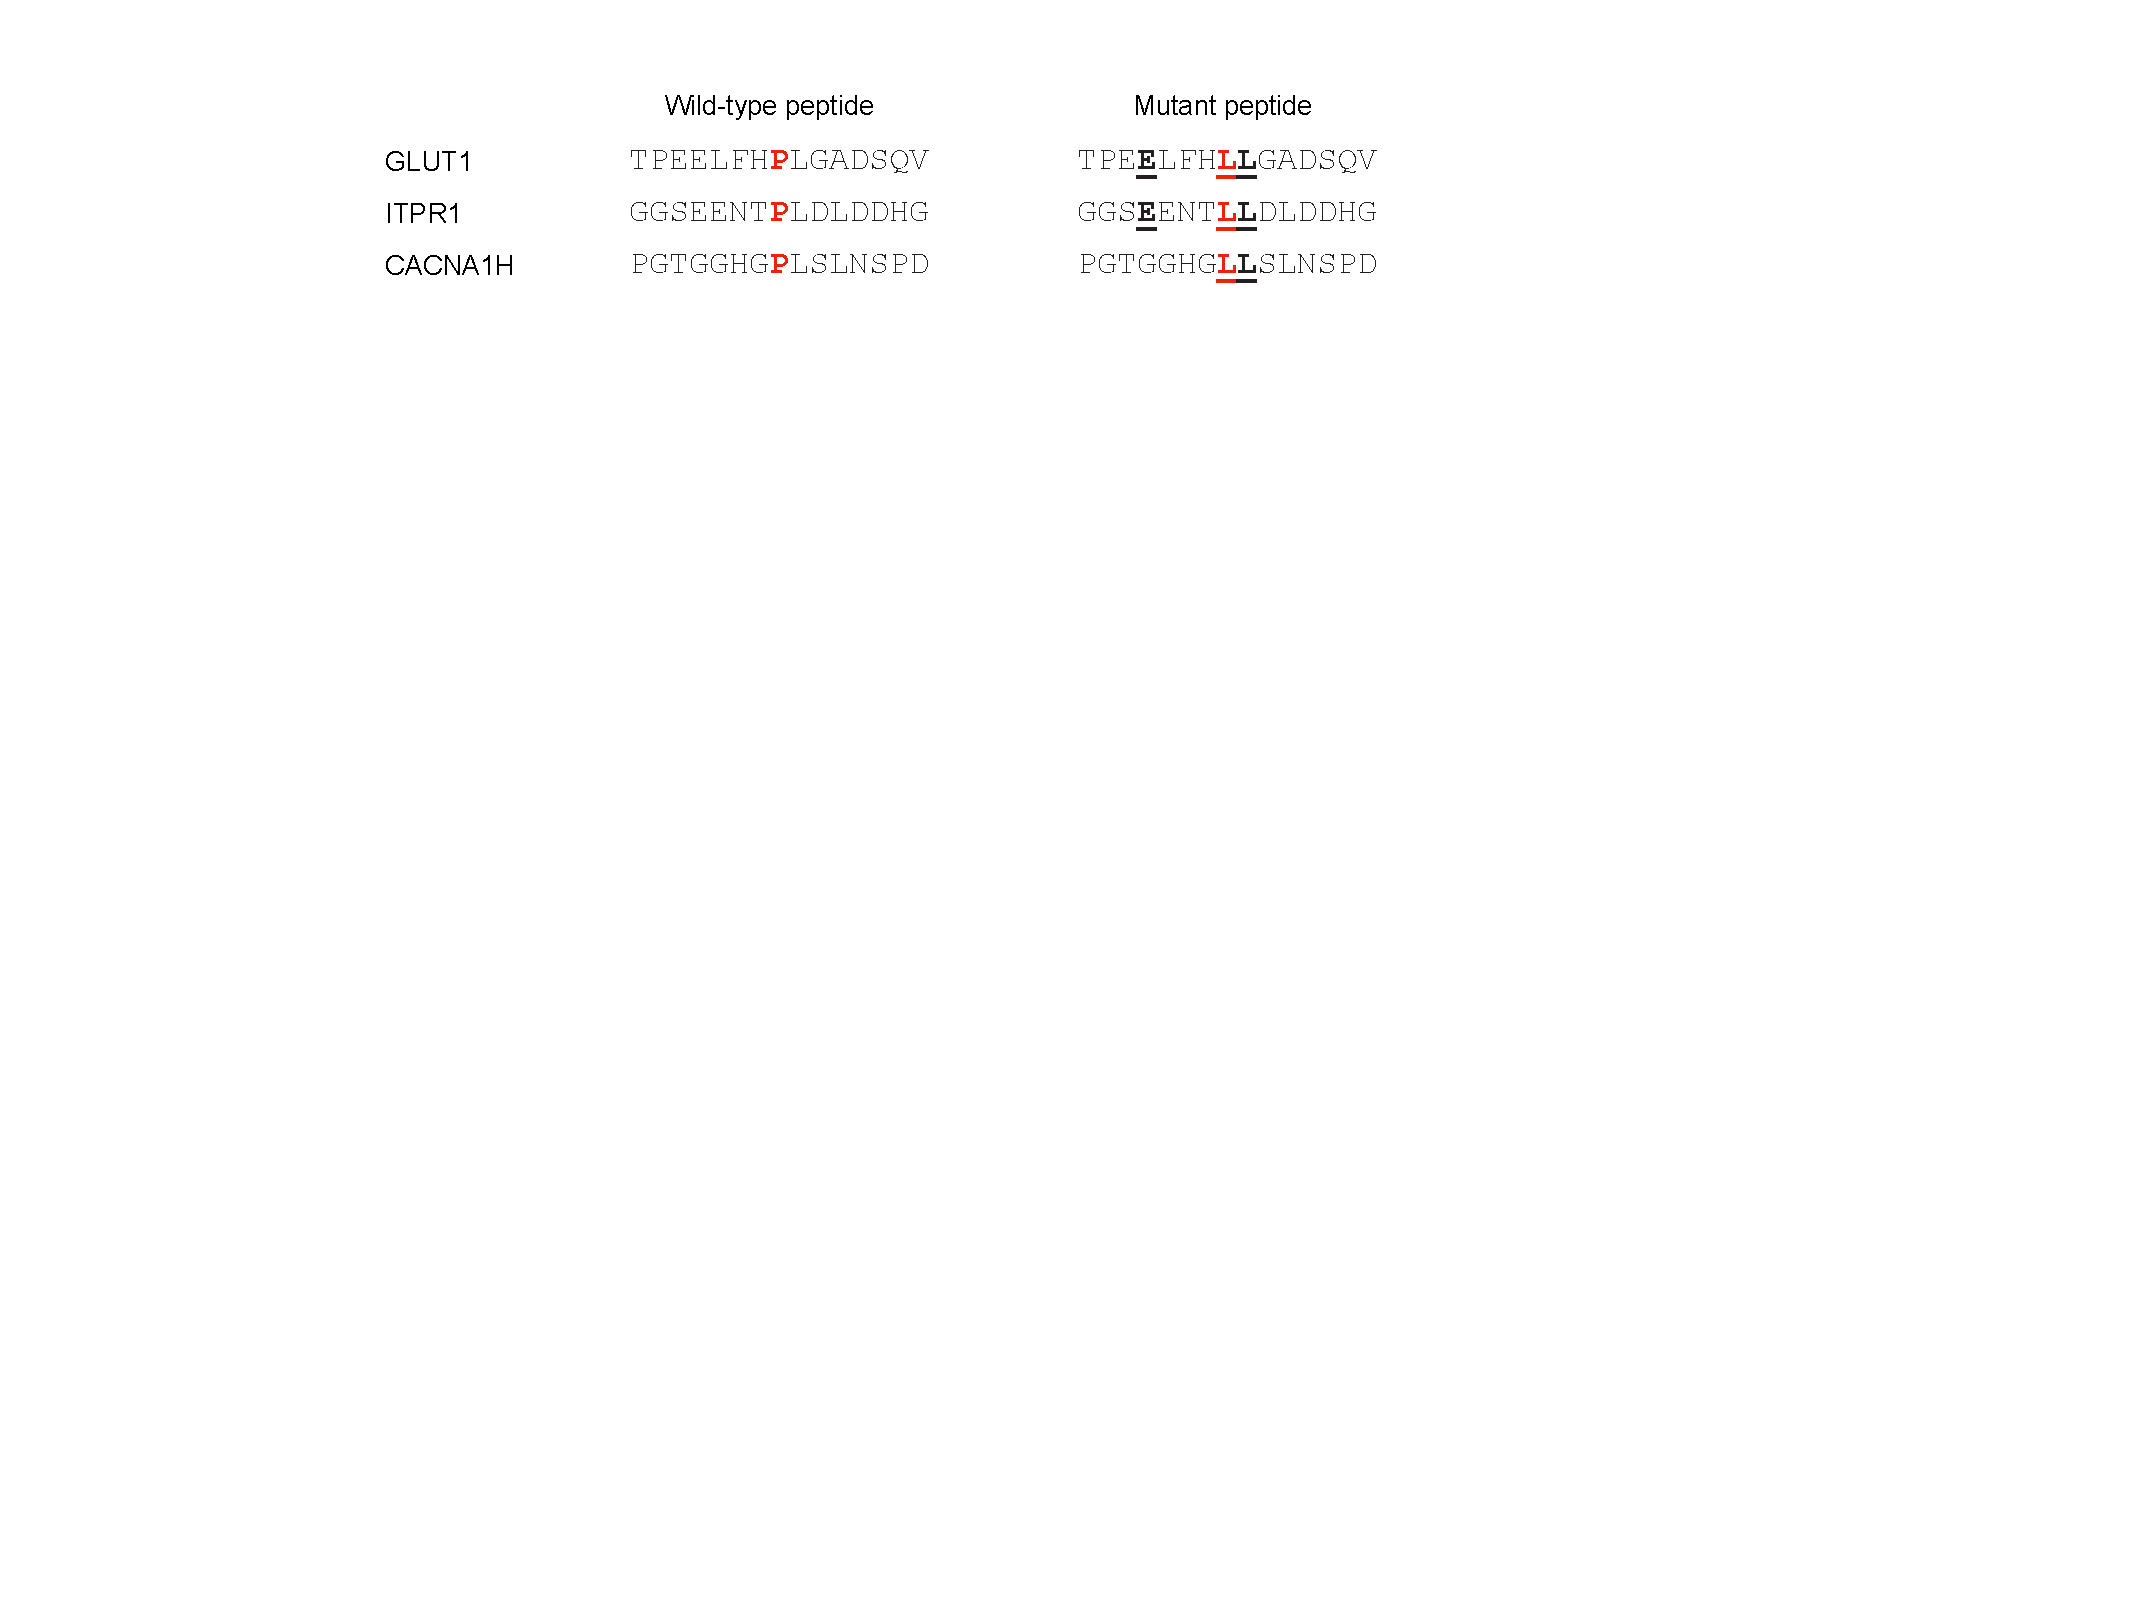
\includegraphics[scale=0.7]{Figures/motif}
\caption{Gain of dileucine motifs in the mutated peptides.}
\label{fig:motif}
\end{figure}

%TPEELFHLLGADSQV
% [D/E]XXXL[L/I] 

%A previous study of the group combined high-throughput peptide pull-downs and quantitative mass spectrometry~\cite{Meyer} to study binding profiles of proteins with disease related mutations. The results have shown that a peptide on the carboxyl terminal of GLUT1 with Pro485-to-Leu mutation (TPEELFHLLGADSQV) binds with clathrin, and this interaction is absent in the binding profile of the wild type peptide. Accordantly, the mutation creates a short linear motif (E...LL) in the cytoplasmic tail region of GLUT1 that interacts with adaptor proteins such as APs and mediates clathrin-dependent endocytic sorting~\cite{Traub}. Furthermore, a proximity-dependent biotin identification (BioID) experiment~\cite{Roux} in HEK293 cells transiently transfected with GLUT1 provides additional evidence for the novel interaction between the mutant GLUT1 and several proteins involved in the clathrin-mediated endocytosis pathway.

\section{Clathrin-mediated endocytosis and intracellular trafficking}
Based on these findings, it is hypothesized that the GLUT1\textsuperscript{P485L} mutation causes clathrin-mediated endocytosis and possibly subsequent degradation of GLUT1, leading to the development of GLUT1-deficiency syndrome. The hypothesis will be further investigated in this master thesis.

% Define some commands to keep the formatting separated from the content 
\newcommand{\keyword}[1]{\textbf{#1}}
\newcommand{\tabhead}[1]{\textbf{#1}}
\newcommand{\code}[1]{\texttt{#1}}
\newcommand{\file}[1]{\texttt{\bfseries#1}}
\newcommand{\option}[1]{\texttt{\itshape#1}}


